%%
%%  This is a LaTeX template for an astronomy Bachelor's thesis.
%%
%%  Version 1.0
%%
%%  Authors: Anders Johansen, Sofia Feltzing, Johan Bijnens (2014)
%%  Send feedback to Anders Johansen <anders@astro.lu.se>
%%
\documentclass[12pt]{report}

\usepackage{a4wide}
\usepackage{graphicx}
\usepackage{natbib}
\usepackage[T1]{fontenc}  
\usepackage[utf8]{inputenc} 
\usepackage{geometry}
\usepackage[justification=centering]{caption}
\usepackage{subcaption}

\usepackage{fancyhdr}
\usepackage{lastpage}
\usepackage{pdfpages}
\usepackage{url}

\pagestyle{fancy}
%\rhead{}
%\chead{}
%\lhead{}
%\rfoot{}
\cfoot{\thepage}
%\lfoot{}

\newcommand{\apj}{ApJ}
\newcommand{\apjl}{ApJ}
\newcommand{\mnras}{MNRAS}
\newcommand{\aap}{A\&A}
\newcommand{\aj}{AJ}
\newcommand{\nat}{Nature}
\newcommand{\pre}{Phys.~Rev.~E}
\newcommand{\araa}{ARA\&A}
\newcommand{\icarus}{Icarus}

\begin{document}

\title{\huge \bf Multiplanetary Systems from Simulated TESS TTV Signals\footnote{This is just a very basic cover page produced by LaTeX -- when
the thesis is done you can get a more formal cover page from Eva Jurlander.}}
\author{Lucas Hellström}

\thispagestyle{empty} % do not count pages just yet

\maketitle

\newpage

\thispagestyle{empty}

\begin{center}
  (this page will contain some more official information in the final version)
\end{center}

\newpage

\thispagestyle{empty}

\begin{center}
  {\bf Abstract}
\end{center}
The abstract is a short summary describing the content of the main text. This
should give enough information about the contents to decide for the intended
audience whether further reading will be useful. The size should be about half
a page, best written at the end, after most of the thesis is written.

\newpage

\thispagestyle{empty}
\mbox{} % this is how we create an empty page in LaTeX

\newpage

\thispagestyle{empty}

\begin{center}
  {\bf Popul\"arvetenskaplig beskrivning}
\end{center}
	När vi letar efter exoplaneter finns det ett antal olika metoder för att hitta dem. Den mest framgångsrika är transitmetoden där ljusstyrkan hos en stjärna studeras under en längre tid. När en planet passerar mellan sin stjärna och en observatör kan en minsking i stjärnans ljusstyrka ses. Uppreras detta i regelbunda intervall kan slutsatsen att det finns en planet runt stjärnan. Genom att studera minskningen i ljusstyrka kan storleken på planeten beräknas vilket kombinerat med massan som fås av andra metoder ger en insikt i hur och vad planeter är uppbygd av. En transit är detta fenomen då en planet passerar mellan stjärnan och en observatör.
	
	Genom att jämföra tiden mellan varje transit för en planet kan ibland variationer ses. Detta beror på att det finns fler planeter runt stjärnan som med hjälp av gravitationskraften accelererar eller decelerera planeten som bevakas. Detta resulterar i att det är möjligt att hitta planeter som i andra metoder är osynliga. 
	
	Keplerteleskopet är ett rymdbaserat teleskop som använder transitmetoden för att hitta exoplaneter. Det har sedan 2009 hittat över 1000 bekräftade exoplaneter vilket gör den till det hittils mest framgångsfulla upgradet i jakten på exoplaneter. TESS, vilket står för Transiting-Exoplanet Survet Satellite, är ett teleskop som ska skjutas upp under våren 2018 och använda transitmetoden för att hitta exoplaneter. TESS kommer bli den första rymdbaserade teleskopet att studera hela himlen och kommer observera över 200 000 stjärnor under uppdragets upsrungliga längd på två år.
	
	Detta projekt kommer använda data från Keplerteleskopet och simulera data från TESS för att sedan använda den datan för att leta efter TTV. Detta ska ge en uppfattning om hur många system har fler än en planet och resultatet kommer kunna ses som en katalog över multi-planet system vilket kan underlätta framtida forskning där en katalog av detta slag kan vara till användning.
	
	


%This is meant to be popular {\it introduction to} and {\it description of} your
%thesis, preferably written in Swedish. The name is unfortunately misleading. It
%is not a summary but mainly an introduction to what you have done. A good idea
%is to write this when you are about one third through the time allotted for the
%thesis work.
%\\ \\
%Especially important here are the context of your project and why this is an
%interesting project to do. This should be about half a page as well.
% Swedish letters: \"a, \"o, \aa

\newpage

\thispagestyle{empty}
\mbox{} % make sure that TOC starts on a right page

\newpage

\setcounter{page}{1} % start counting pages

\tableofcontents

\newpage

\listoffigures 
\listoftables

\newpage

\chapter{Introduction}

This document is meant as a technical tutorial for writing an
astronomy/astrophysics thesis in LaTeX. Detailed rules about the {\it contents}
of the thesis (Bachelor's thesis or Master's thesis) can be found at the course
websites.

\section{Transits}
	A planet in orbit around it's host star may sometimes cross the line of sight of an observer. When this happens a slight decrease in the stars brightness can be measured. This is called a transit and is today used as a main method to discover exoplanets. From transits the radius of the planet can be determined but it can also be used to find additional planets around the host star which may not be transiting. This will be discussed in section \ref{sec:trans_vari}. With the radius known from the transit method and the mass obtained from different methods as the radial velocity method the density of the planet can be calculated. The density is important to understand what the planet is made of and the structure of it.

\subsection{Variations}
\label{sec:trans_vari}

	When measuring the time of one transit one may discover variations in the period which are called Transit-Timing Variations or TTVs. These variations arise from another planet in the system whose gravitational pull accelerates or decelerate the observed planet which results in increased or decreased transit times. An advantage of studying transits in search for TTVs is that planets which does not transit their star can be discovered through TTVs. As most planets does not transit their star this can increase the number of known exoplanets drastically.

\section{Kepler}
	The Kepler satellite launched in spring 2009 on a mission to study stars in a small patch in the sky to discover Earth-sized exoplanets within the habitable zone, where liquid water can exist on the planetary surface. The brightness of a large amount of stars are measured and then analyzed in order to detect transiting exoplanets.
	
	Kepler started by looking at a very small patch of the sky but in July 2012 one of the four wheels used to keep the patch in focus broke. The telescope requires at least three wheels to function which kept the mission alive. In May 2013 a third wheel failed which resulted in the telescope no longer being able to collect data. The satellite was nonfunctional until the so-called "Second Light (K2)" in early 2014. This mission would use the telescopes remaining two wheels to study stars over a much larger area but for shorter periods.
	
	According to \cite{kepler_num_planet} Kepler found over 2300 confirmed exoplanets and about 2200 candidates which require further studies before they can be confirmed during the main mission, before the second wheel broke down. Since the start of K2 about 300 exoplanets have been confirmed and close to 500 candidate exoplanets. These numbers makes Kepler the most successful exoplanet hunting mission to this date.
	
	
\section{TESS}
	The Transiting Exoplanet Survey Satellite, TESS, is a satellite due to launch spring 2018. The satellite is equipped with four cameras which will study the brightness of over 200 000 stars over a two year period. It is the first all-sky transit survey taking place in space.
	
	TESS will cover the whole sky by splitting it into 26 sectors which are observed for 27 days each. An illustration of this can be seen in figure \ref{fig:tess_time} where the number of times TESS will observe each sector is shown. 
	\begin{figure}[h!]
	\centering
		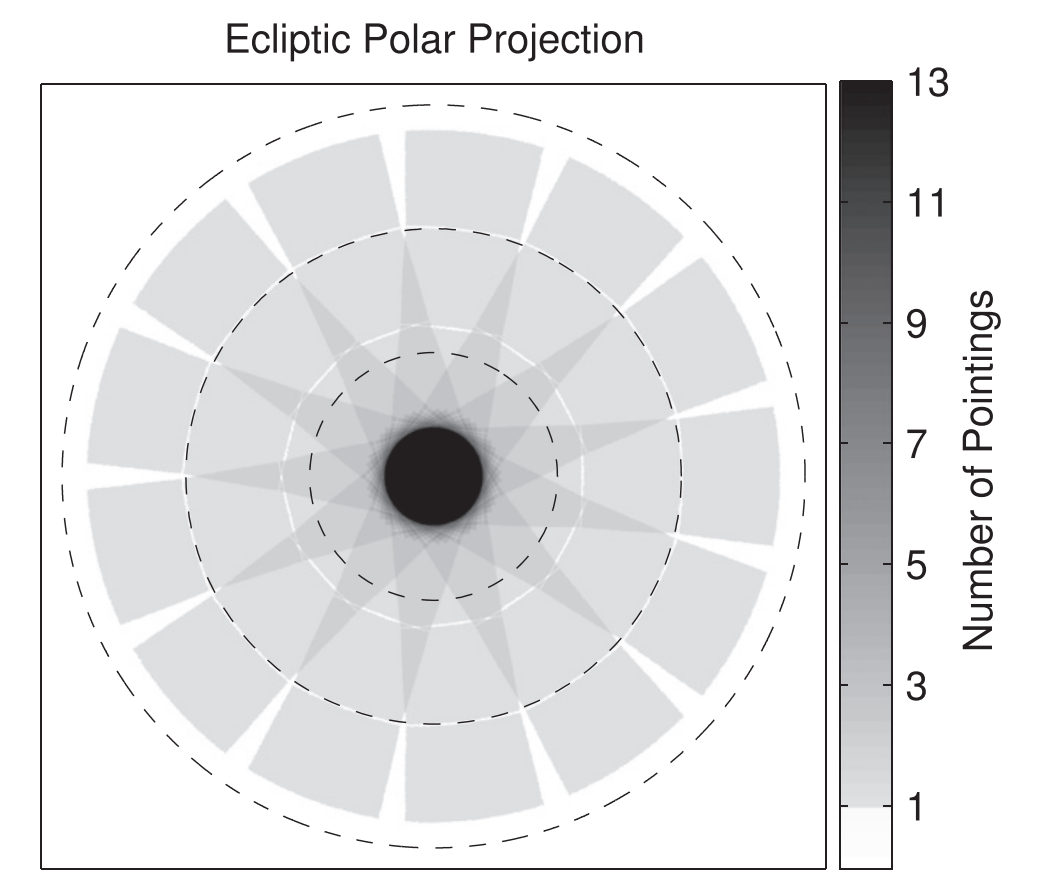
\includegraphics[scale=0.2]{img/tess_observe_time.png}
		\caption{Illustration of the number of times TESS will observe each sector in the sky.\\ \small{Source: \cite{2015ApJ...809...77S}}}
		\label{fig:tess_time}
	\end{figure}
	%

\chapter{Method}

\section{Simulation of TESS objects}
	By combining data from Kepler obtained from the NASA Exoplanet Archive and the results from \cite{2015ApJ...809...77S}, which contains one planet for each system, TESS data are simulated. For each planet in the Sullivan catalogue, a similar planet, in radius and period, are found in the NASA archive. The ratio of radius and period are calculated and applied to the Kepler planet to make it identical in radius and period to the Sullivan planet. This ratio is then applied to any other planets in the Kepler system to make an artificial system of planets. Another parameter when finding planets in the NASA archive is the effective temperature of the star in the system. The systems are divided into two groups where one have effective temperatures of over 4000 kelvin and the other are below. This is to ensure that one system with a small, cool star is not combined with a system containing a big, hot star.   (\textbf{picture?})

\section{TTVFast}
	TTVFast is a program created by \cite{2014ApJ...787..132D} which simulates planetary systems. It uses a number of parameters:
	\begin{itemize}
		\item Gravitational constant in $AU^3 \mathrm{day}^{-2}M_{\odot}^{-1}$
		\iffalse \item Time step which is recommended to be $1/20$ of the shortest period in the system.
		\item Reference time where the integration should start. $T_0 = 0$ is used in this paper.
		\item Final time where the integration should stop. This is obtained from the Web TESS Target tool where the right ascension and declination of each system is given and the corresponding times TESS will look at each system is given back.(https://heasarc.gsfc.nasa.gov/cgi-bin/tess/webtess/wtm.py)
		\item Number of planets where all planets should be included even if they aren't transiting.
		\item \fi
	\end{itemize}

\section{Analyzing results from TTVFast}



\chapter{Results}

\iffalse Chapters always start on a new page. The chapter names in the template are just
suggestions. You can name your chapters differently and add more if needed.

\begin{verbatim}

       PROGRAM myfortran

       IMPLICIT NONE

       REAL*8 mag(20)
       REAL flux(20)
       INTEGER nstar

       WRITE(*,*) "This program calculates a magnitude"
       READ(*,*) flux(1)
       mag(1)=-2.5*LOG(flux(1))

\end{verbatim}
\fi

\section{Simulated TESS objects}



\begin{figure}
 	 \centering
 	 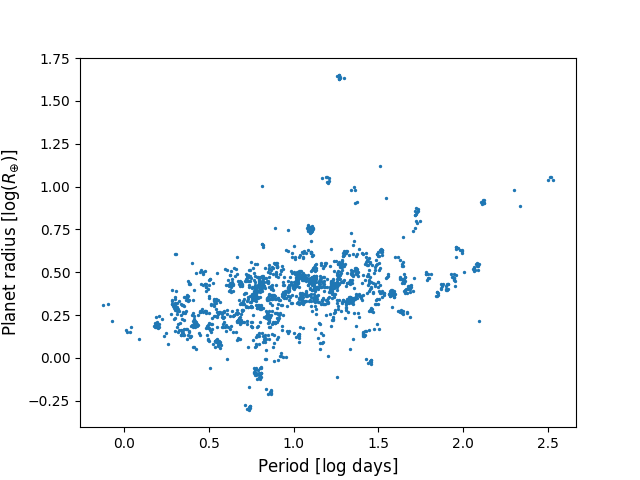
\includegraphics[width=9cm]{img/R_P-plot_5.png}
 	 \caption{Diagram with the radius \\distribution as a function of period forthe simulated TESS objects.}
 	 \label{fig:RP_plot}
\end{figure}

\begin{figure}
 	 \centering
	  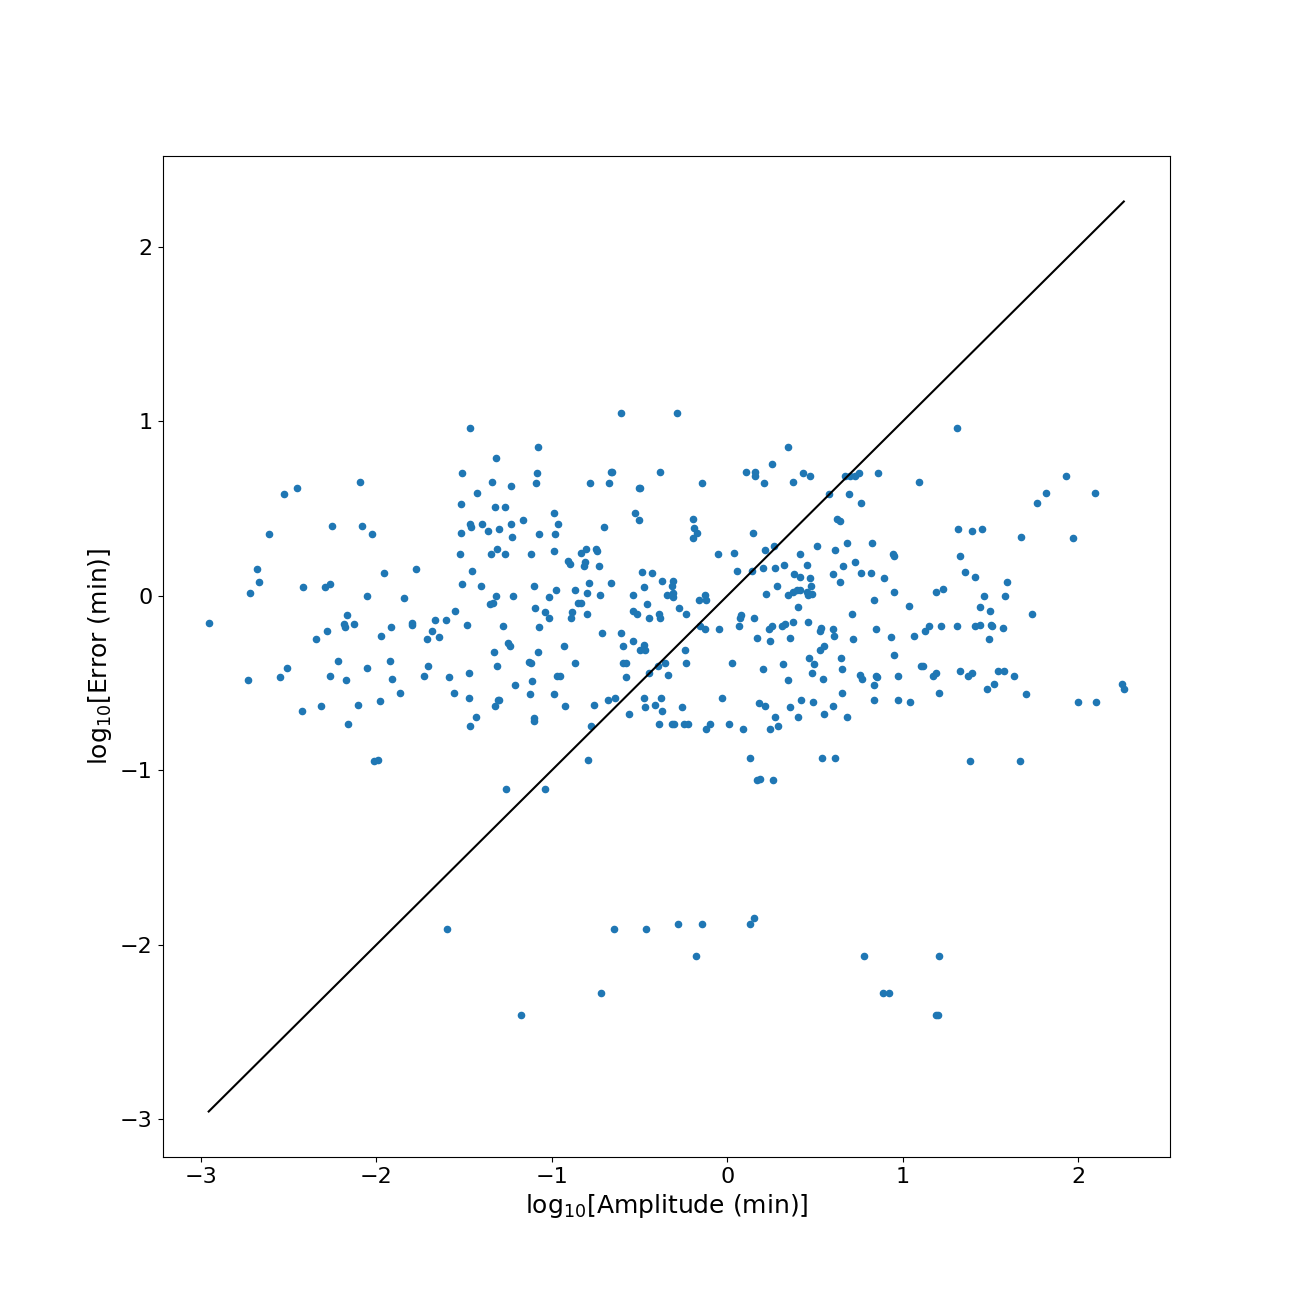
\includegraphics[width=9cm]{img/ampErrorLog.png}
	  \caption{Diagram with the position of each observed objects color-coded to show the number of times the object is observed.}
	 \label{fig:pos_num_obs}
\end{figure}

	\begin{figure}
		\centering
		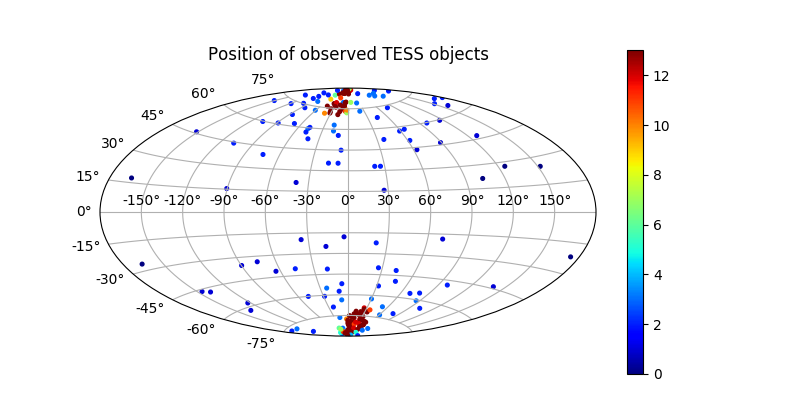
\includegraphics[width=12cm]{img/skymap_TESS_wrap.png}
	  	\caption{Diagram with the position of each observed objects color-coded to show the number of times the object is observed.}	
	  	\label{fig:skymap_TESS}	
	  \end{figure}

\section{TTV signals from TESS objects}


\begin{table}[!h]
\caption{Example table from template}\smallskip
\label{table:1}
\centering  
\begin{tabular}{lrrc}
\hline\hline  
\smallskip
Id of star & I &  V & Var.? \\
\hline
1234 & 15.6 & 17.3 & No \\
5677 & 13.4 & 12.3 & Yes\\
\hline
\end{tabular}
\end{table}

\chapter{Discussion}
	Further studies: CHEOPS, James Webb
\chapter{Conclusions}


\section*{Acknowledgements}

There is no acknowledgements section in the regular LaTeX, but you can easily
make one yourself.

%\bibliographystyle{natbib}
%\begin{thebibliography}{99}
%\bibitem[Alexander \& Armitage(2007)]{2007MNRAS.375..500A}
%  Alexander, R.~D., \& Armitage, P.~J. 2007, \mnras, 375, 500
%\bibitem[Santos et~al.(2001)Santos, Israelian, \& Mayor]{2001A&A...373.1019S}
%  Santos, N.~C., Israelian, G., \& Mayor, M. 2001, \aap, 373, 1019
%\end{thebibliography}

\bibliographystyle{aa}
\bibliography{references}

\begin{appendix}

\chapter{This is an appendix}

You can put long mathematical derivations or tables in appendices.

\chapter{This is another appendix}

\end{appendix}

\end{document}
